%%%%%%%%%%%%%%%%%%%%%%%%%%%%%%%%%%%%%%%%%%%%%%%%%%%%%%%%%%%%%%%%%
%  _____   ____  _____                                          %
% |_   _| /  __||  __ \    Institute of Computitional Physics   %
%   | |  |  /   | |__) |   Zuercher Hochschule Winterthur       %
%   | |  | (    |  ___/    (University of Applied Sciences)     %
%  _| |_ |  \__ | |        8401 Winterthur, Switzerland         %
% |_____| \____||_|                                             %
%%%%%%%%%%%%%%%%%%%%%%%%%%%%%%%%%%%%%%%%%%%%%%%%%%%%%%%%%%%%%%%%%
%
% Project     : LaTeX doc Vorlage für Windows ProTeXt mit TexMakerX
% Title       : 
% File        : anhang.tex Rev. 00
% Date        : 7.5.12
% Author      : Remo Ritzmann
% Feedback bitte an Email: remo.ritzmann@pfunzle.ch
%
%%%%%%%%%%%%%%%%%%%%%%%%%%%%%%%%%%%%%%%%%%%%%%%%%%%%%%%%%%%%%%%%%


%\pagenumbering{Roman}

%\appendix
\chapter{Appendix}\label{chap.anhang}

If you are interested in the source code of this work, you can reach us at:\\dano.roost@gmail.com or ralphlmeier@gmail.com

\section{USB Flash Drive Content}

The attached USB flash drive contains the following content:
\begin{itemize}
    \item This report as PDF
    \item The source code of all experiments
    \item The source code of the final training (final state)
    \item The best submission for round 1 and round 2
    \item A readme file
\end{itemize}

\section{Official assignment}

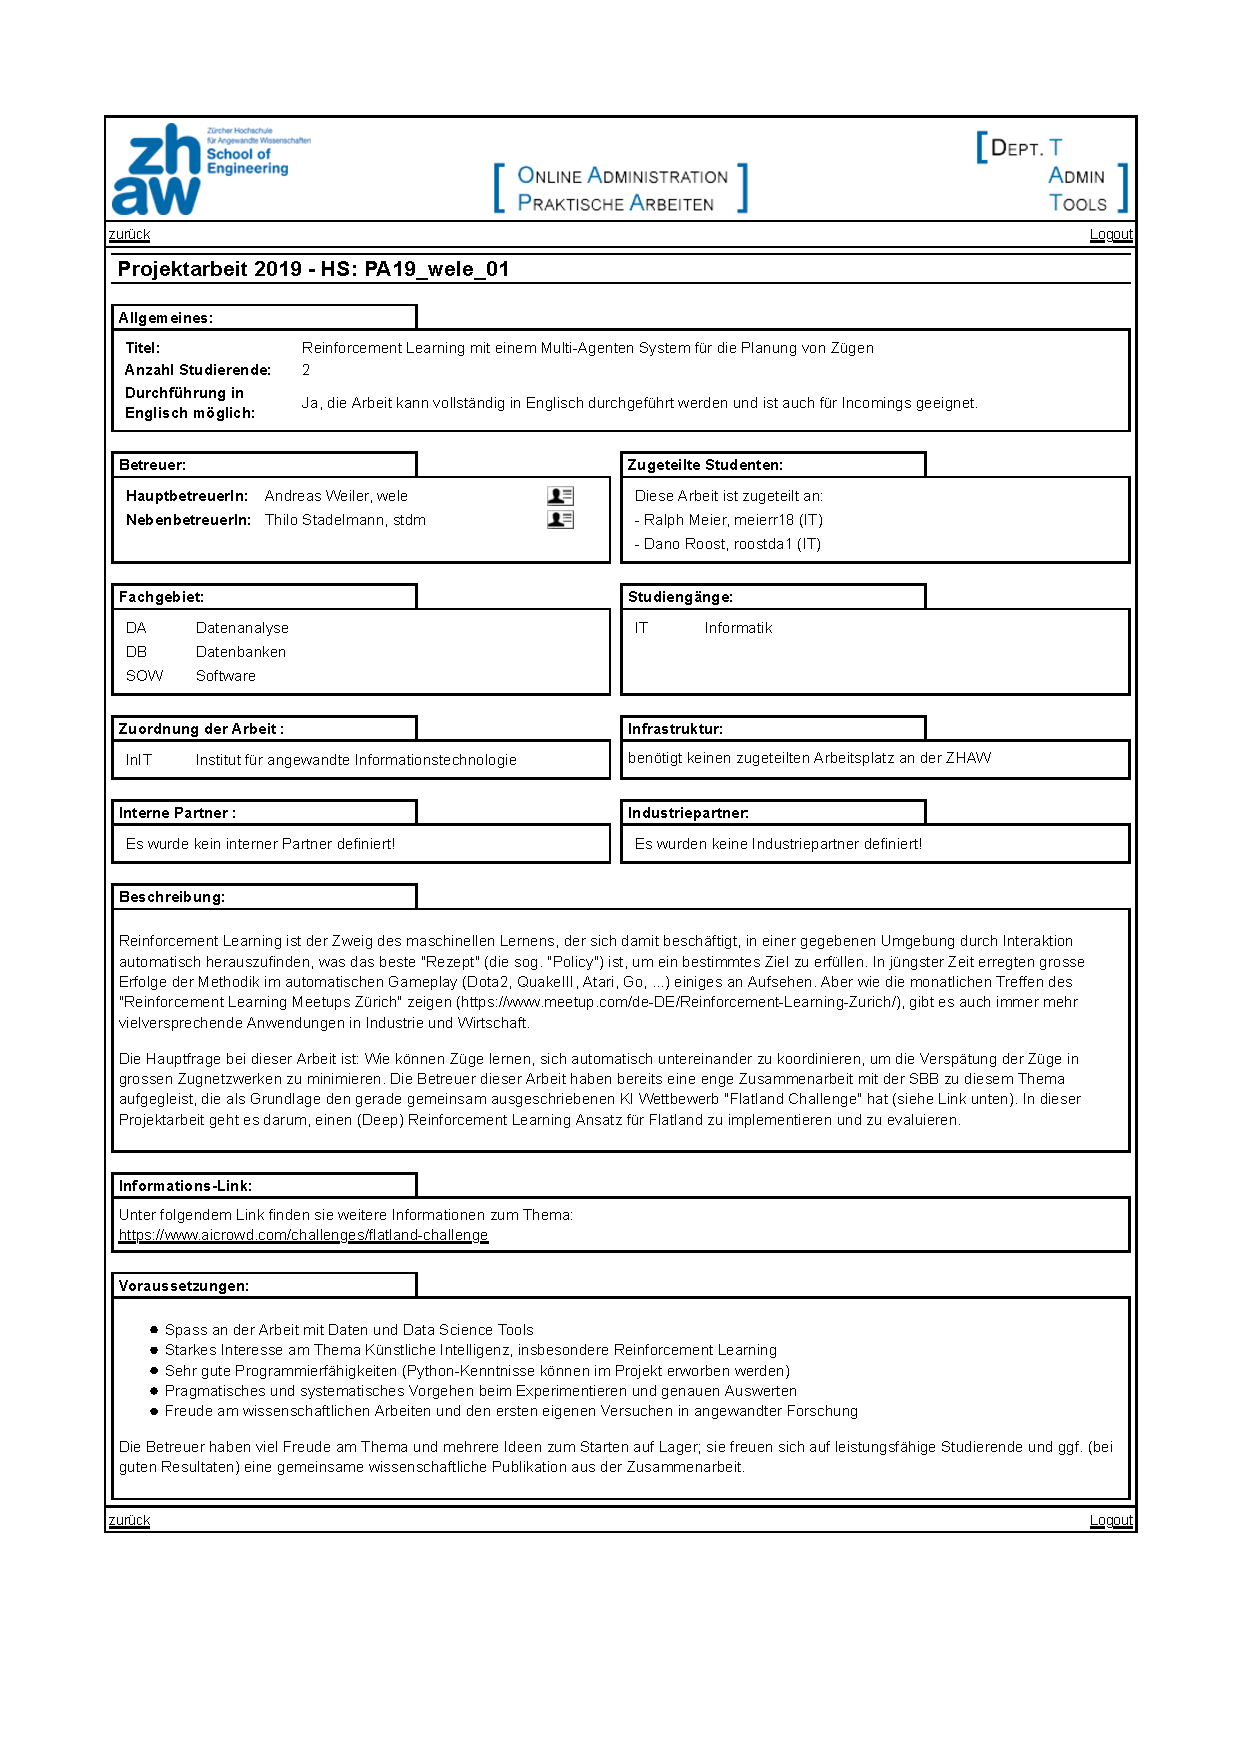
\includepdf{images/PA_Aufgabenstellung.pdf}

\NewPage